\section{Aims}
% general intro
\red{TODO: general intro?}
% new statistical aligner that combines robust models of sequences evolution
%  with models capable of handling artifacts caused by genome sequencing and
%  assembly errors.
% called COATI (COdon-aware Alignment Transducer)
% suited for all types of aln problems, including non-coding DNA

\subsection{Statistical Pairwise Alignment of Protein Coding Sequences}
% Talk about pairwise alignment

% pair-HMM vs FSTs.
\red{TODO: reword (reorder?) so that is not so similar to grant.}\\
\subsubsection{Pairwise hidden Markov models pair-HMMs.}
Statistical alignment is typically performed using pair-HMMs.
Pair-HMMs are computational machines with two output tapes, commonly a finite
number of states that emit symbols onto one or both tapes.
When applied to sequence alignment, the states are \green{usually classified
or categorized} as match, insertion, and deletion and the emitted symbols can be
nucleotides or amino acids.

A path through the pair-HMM represents a possible alignment between the
sequences.
Conceptually, these machines generate two sequences ($X$ and $Y$) from some
common unknown ancestor ($Z$) and calculate $P(x,z) = \sum_y P(x,y,z)$
\parencite{yoon_2009_hmm}.
Pair-HMMs can rigorously model molecular sequence evolution, calculate the
probability that two sequences are related (Forward algorithm), estimate optimal
alignment (Viterbi), and estimate model parameters (Baum-Welsch).

\subsubsection{Finite state transducers (FSTs)}
A limitation of pair-HMM is the ability to only model evolution of two related
sequences from an unknown ancestor, not being able to use the output of one
pair-HMM as the input of another pair-HMM.
\green{Finite-state transducers (FSTs) share/include the same
probabilistic/computational benefits as pair-HMMs except that have an input and
output tape, instead of two output tapes.}
It absorbs symbols from an input tape and emits symbols to an output tape.
Conceptually, an FST generates a descendant sequence given an ancestral one
$X \Rightarrow Y$.
Properly weighted, an FST can calculate the conditional probability that
sequence $Y$ evolved from seq $X \rightarrow P(y|x)$).

FSTs have similar benefits to pair-HMMs in addition to well established
algorithms for combining them in different ways \red{citation}.
A \green{key/popular/essential/important/powerful} example is composition, which
consists of sending the output of one FST as the input of a second one.
This allows $P(Z|X) = \sum_Y P(Z|Y) P(Y|X)$, represented $X \Rightarrow$ any
$Y$ $\Rightarrow Z$.
In the development of COATi I will design complex FSTs from smaller FSTs, each
representing a specific process.

\begin{center}
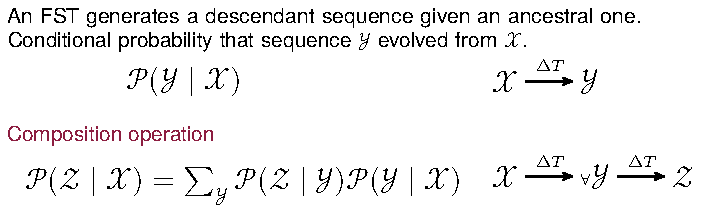
\includegraphics[scale=1]{figures/fig-fst.pdf}
\end{center}

\subsubsection{Evolution FST}

% evolution fst intro
The evolution FST is based on existing transducers \red{citation}.
This FST is formed by composing a substitution FST that models codon
substitutions and an indel FST that models insertions and deletions, including
frameshifts.
The power of this FST with respect to others is the combination of a codon
substitution model with gaps that can occur at any position and of any length.

% TODO: change substitution FST to not be marginal model
\begin{figure}
\centering
    \hspace*{-2cm}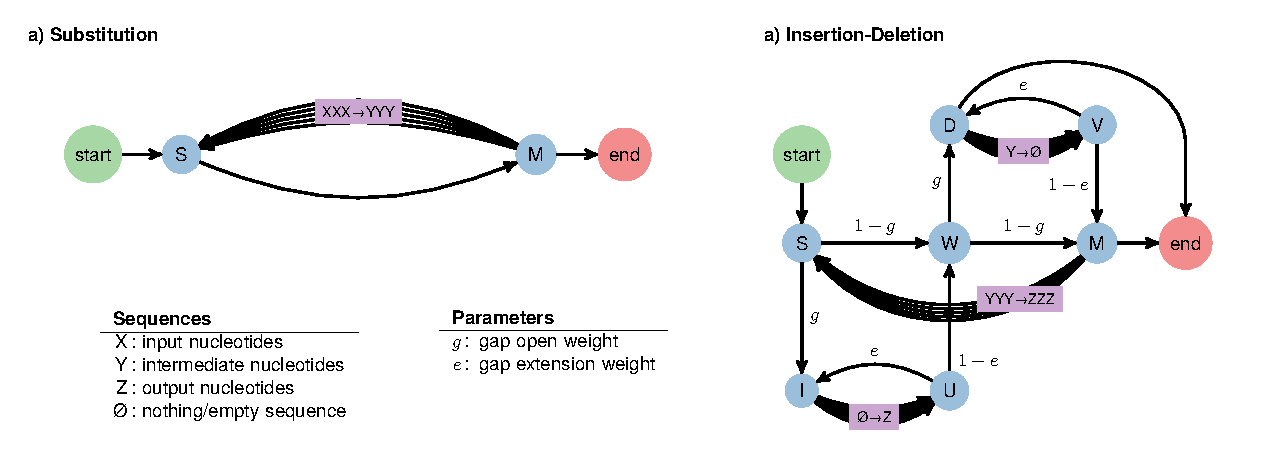
\includegraphics[width=\textwidth]{figures/fig-evolution-fst.pdf}
    \caption{Substitution FST and indel FST. Both Mealy machines, consuming or
    emitting characters during transitions between states. Substitution FST will
    match an input codon with a codon output.
    Indel FST allows gaps at any position and guarantees insertions to precede
    deletions to limit equivalent alignments.}
\centering
\end{figure}

\textbf{Substitution model.}
% substitution model
Despite the availability of codon models, vastly used in phylogenetics, sequence
alignment has not benefited from these advancements.
COATi will support an abundance of codon models by using a continuous-time
Markov model, with instantaneous substitution rate matrix $Q$:
%  Q matrix
\begin{align*} Q_{ij} &= \begin{cases}
    \mu_{ij} & \text{if $i$ and $j$ are synonymous}\\
    \omega \cdot \mu_{ij} & \text{if $i$ and $j$ are nonsynonymous}
    \end{cases}\\[10pt]
   Q_{ii} &= -\sum_{j:j \neq i} Q_{ij}
\end{align*}

where each position in $Q$ defines the rate that codon $i$ changes to codon $j$
and main diagonal elements are calculated so that total rate for each row is 0.
Model parameter $\mu_{ij}$ is the mutation rate of codon $i$ to $j$ and $\omega$
represents the strength of selection for amino acid changes.
The substitution probability after time $t$ is calculated via matrix
exponentiation $P(j|i;t) = e^{Qt}$.

% different ways to select parameter values
COATi will offer different ways to specify mutation rates ($\mu$), including
implemented models such as Muse and Gaut (MG94) \red{citation}, empirical codon model
\red{citation}, and specified by user via an input file.

% summary paragraph
\textbf{COATi alignpair.}
Evolution FST is a powerful statistical pairwise aligner that benefits from
robust and modern codon models while allowing gaps at any position and offers
the ability to control model parameters such as substitution rates, selection,
and indel distributions.
Coati-alignpair will find the optimal alignment between two sequences (Viterbi
algorithm) and the probability that the sequences are related (Forward algorithm).

\subsubsection{Dynamic Programming}
Composition is one of the most powerful operations on FSTs, as it allows complex
FSTs to be build from smaller and simpler parts.
However, composing many large FSTs is expensive and can be prohibitive.
Despite the existence of efficient C++ FST libraries, runtime is still limiting
when dealing with sequences longer than a few thousand nucleotides.

To solve this issue, the search of an optimal path (alignment) through the
evolution FST can be reformulated as a dynamic programming problem.
Maintaining the statistical framework, COATi will implement a Gotoh-like
thus reducing the problem to a manageable $\mathcal{O}(n \cdot m)$ runtime,
where $n$ and $m$ are the length of the sequences.
This can be further improved by \green{implementing/applying} Myers and Miller
\red{citation}, which sees further time and memory improvement \green{via} a
divide and conquer approach.

\begin{center}
    \hspace*{-3cm}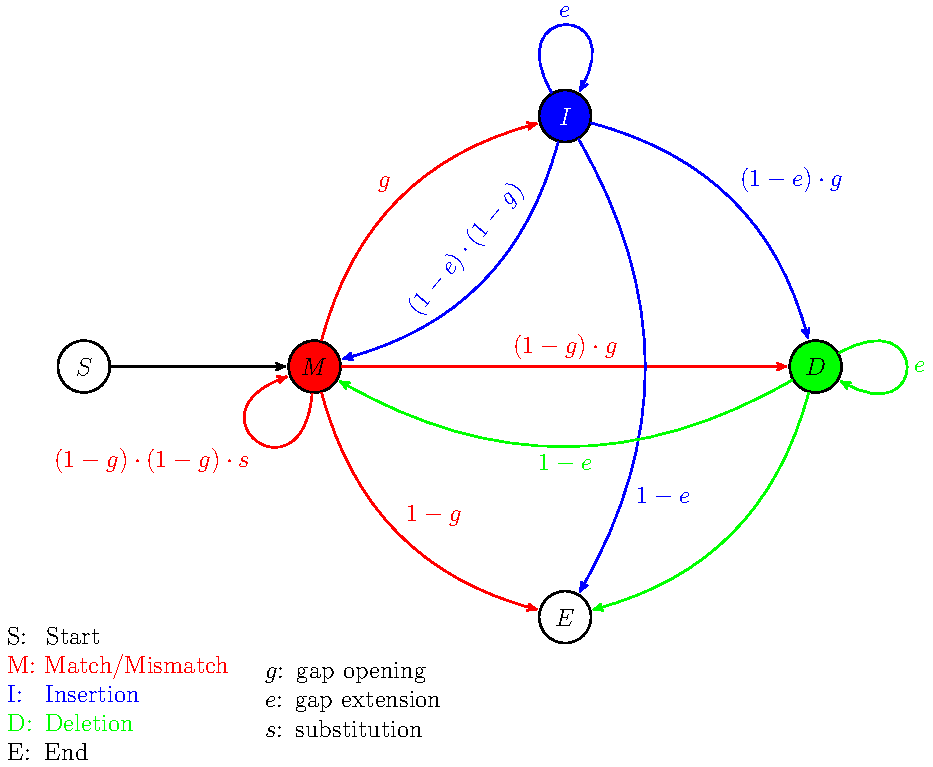
\includegraphics[scale=0.75]{figures/fig-dp-model.pdf}
\end{center}

\subsubsection{Validation}
\textbf{Simulated data.}
% simulated data is an almost mandatory step in every tool validation process
% this will be done by simulating alignments with different values for substitution
%  and indel rates as well as divergence (?)
% To make this step more realistic, gap patterns will be inferred from real data
%  alignments.

\textbf{Real/biological data.}
\begin{itemize}
    \item maybe comment that all current alignment benchmarks are AA?
    \item probably use some "downstream analysis" result for validation (comparison)
\end{itemize}
